\documentclass[12pt]{article}
\usepackage[utf8]{inputenc}
\newcommand\preamble{
    \usepackage[italian]{babel}
    \usepackage{geometry}
    \usepackage{amsmath}
    \usepackage{amssymb}
    \usepackage{graphicx}
    \usepackage{ulem}
    \usepackage[dvipsnames]{xcolor}

    \geometry{margin=2cm}
    \let\olditemize\itemize
    \renewcommand\itemize{\olditemize\setlength\itemsep{0em}}
    \graphicspath{{../Immagini/}}

    \author{Lorenzo Vaccarecci}
}
\preamble

\title{Indici Hash}
\date{5 Aprile 2024}

\begin{document}
\maketitle
L’uso di indici ad albero ha lo svantaggio di richiedere la scansione di una struttura dati, memorizzata su disco, per localizzare i dati. Questo perché le associazioni $(k_{i}, r_{i})$ vengono mantenute in forma esplicita, come record in un file Gli indici hash al contrario mantengono le associazioni $(k_{i}, r_{i})$ in modo implicito, tramite l’uso di una funzione hash, definita sul dominio della chiave di ricerca.
\section{Caratteristiche Generali}
\begin{itemize}
    \item Una funzione hash su $K$ è una funzione \textcolor{red}{surgettiva $H(D_{K})\rightarrow\{0,\dots,M-1\}$}
    \item $M$ costante
\end{itemize}
\begin{center}
    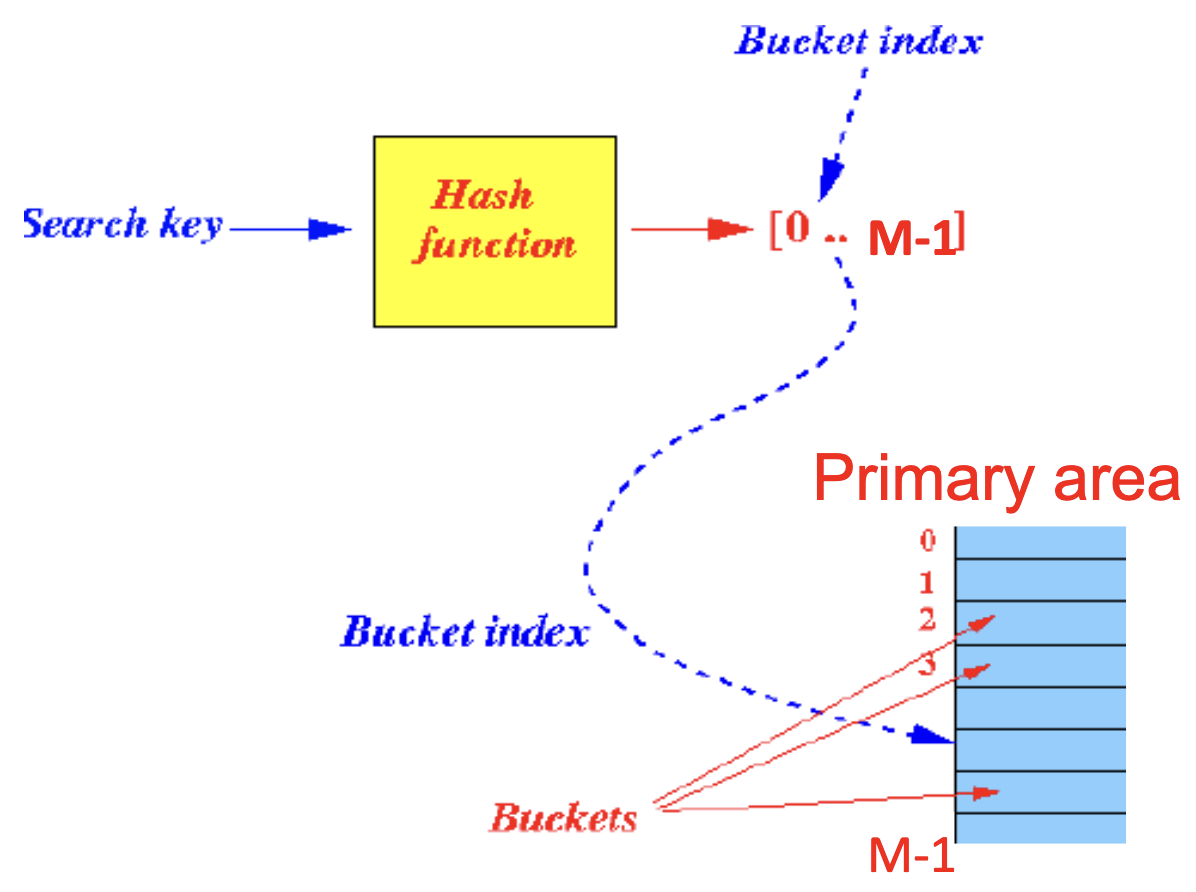
\includegraphics[scale=0.5]{indicihashgen.png}
\end{center}
\textit{A ogni valore della funzione hash corrisponde un indirizzo in area primaria.}\newpage
\subsection*{Esempio}
$I_{A}(R) \quad H(D_{A}\rightarrow\{0,\ldots,2\})$, la funzione $H$ restituisce il numero del bucket.
\begin{itemize}
    \item $H(1)=1$
    \item $H(2)=2$
    \item $H(3)=0$
    \item $H(5)=2$
    \item $H(10)=1$
\end{itemize}
1. creo bucket index: 
\begin{tabular}{|c|c|c|}
    \hline
    0 & 1 & 2 \\
    \hline
\end{tabular}\\
\begin{tabular}{|c|c|}
    \hline
    A & B\\
    \hline
    1 & a \\
    2 & a \\
    3 & b \\
    5 & c \\
    10 & d \\
    3 & f \\
    \hline
\end{tabular} $\Rightarrow$
\begin{tabular}{|cc|}
    \hline
    \textbf{Bucket 0} & \hphantom{}\\
    3 & b\\
    3 & f \\
    \hline
    \textbf{Bucket 1} & \hphantom{}\\
    1 & a \\
    10 & d \\
    \hline
    \textbf{Bucket 2} & \hphantom{}\\
    2 & a \\
    5 & c \\
    \hline
\end{tabular}
\section{Ricerca per uguaglianza}
\begin{center}
    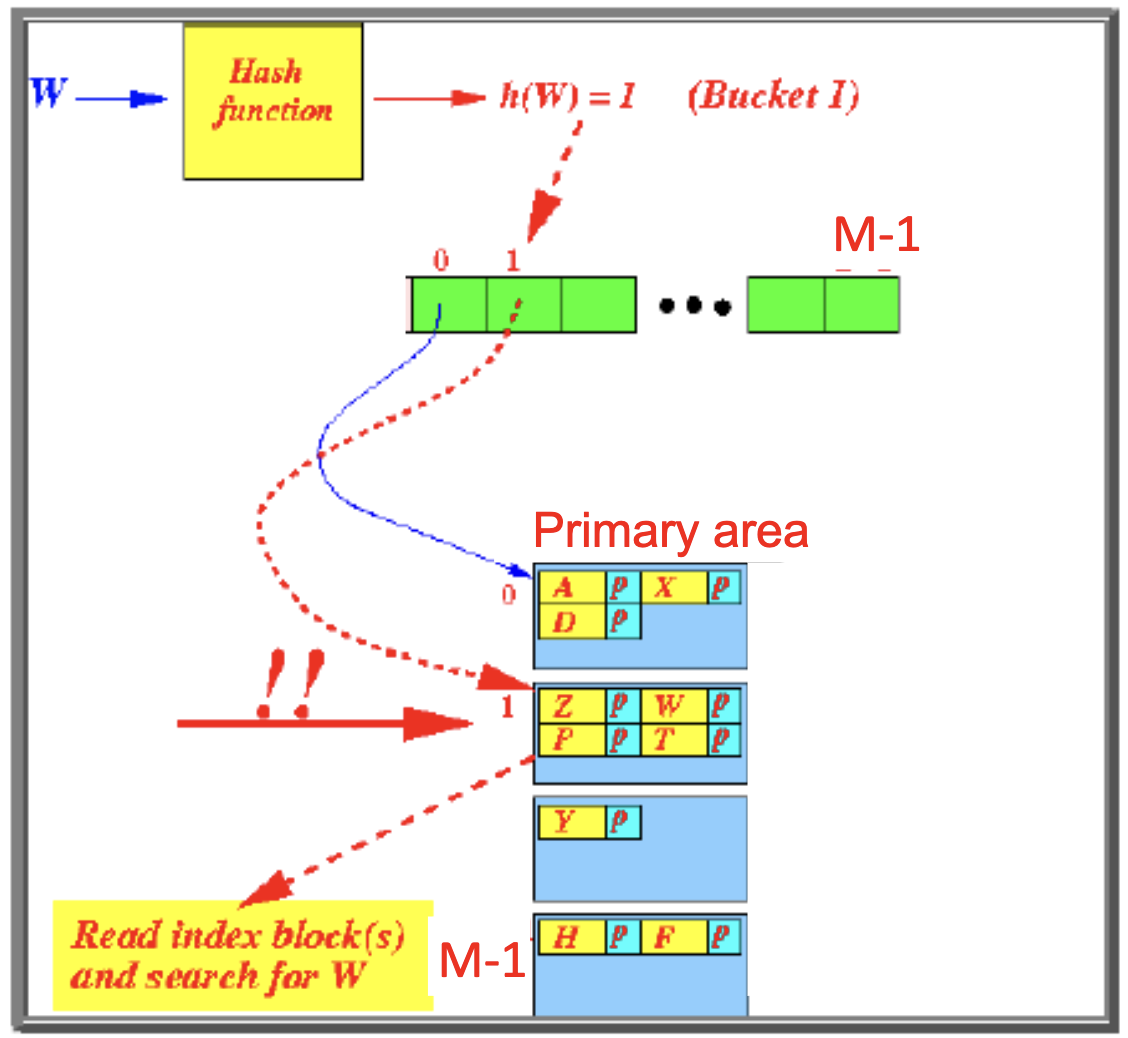
\includegraphics[scale=0.5]{indicihashuguaglianza.png}
\end{center}
\textit{Non supporta la ricerca per intervallo in quanto dovrei conoscere tutti i valori dell'intervallo in quanto la funzione hash non mantiene l'ordine.}
\section{Inserimento e Trabocchi}
\begin{center}
    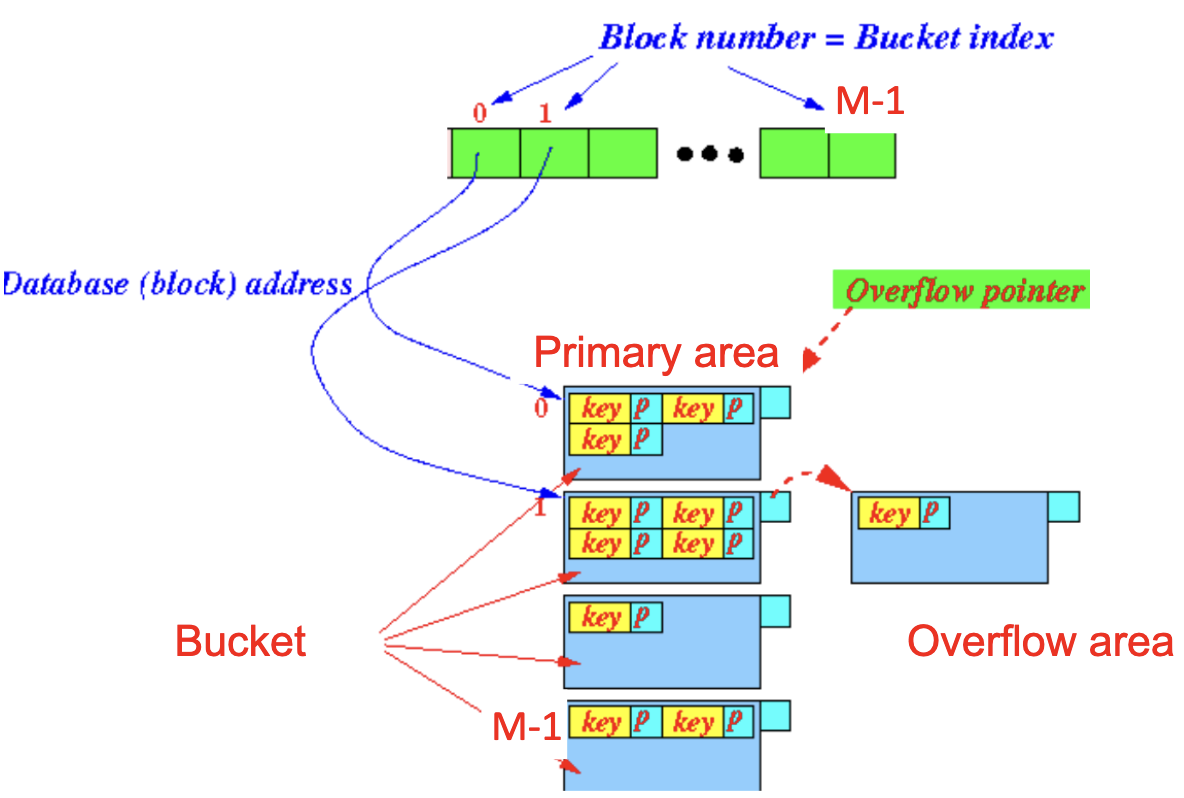
\includegraphics[scale=0.5]{inidicihashinserimento.png}
\end{center}
Se il bucket è pieno, si alloca un nuovo blocco (\textit{trabocco}) dove c'è spazio chiamato \textcolor{red}{area di overflow} e se anche l'area di overflow è piena se ne crea un'altra e così via.
\subsection{Ricerca}
\begin{center}
    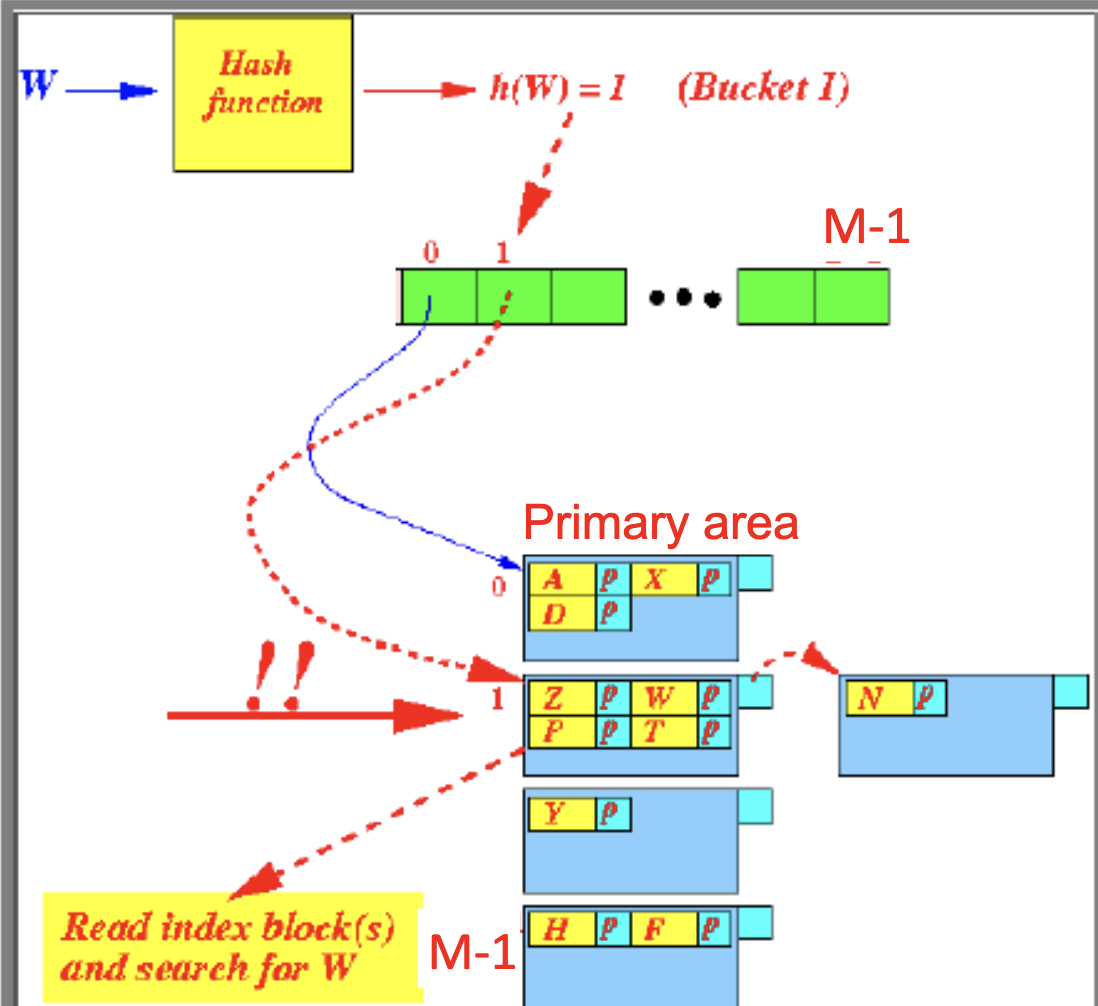
\includegraphics[scale=0.4]{indicihashricercatrabocco.png}
\end{center}
\end{document}